\section{Comparison between tables from Ngspice and Octave} 
\label{sec:comparison}
This section aims to confirm the values between the two analysis. The graphics obtained in both analysis can be viewed side-by-side in section \ref{sec:attachments}.
\subsection{t$<$0}

\begin{table}[h]
\begin{center}
  \begin{tabular}{|c|c|}
    \hline    
    {\bf Name} & {\bf Value [A or V]} \\ \hline
    $I_b$ & -2.658976e-04
$I_c$ & 0
$I_R$$_1$ & 2.536488e-04
$I_R$$_2$ & 2.658976e-04
$I_R$$_3$ & -1.224882e-05
$I_R$$_4$ & 1.205310e-03
$I_R$$_5$ & -2.658976e-04
$I_R$$_6$ & 9.516615e-04
$I_R$$_7$ & 9.516615e-04
$V_1$ & 5.054819
$V_2$ & 4.793705
$V_3$ & 4.258198
$V_4$ & 4.831047
$V_5$ & 5.668298
$V_6$ & -1.934226
$V_7$ & -2.905231
$V_8$ & -1.934226

    \hline
  \end{tabular}
  \begin{tabular}{|c||c|}
    \hline    
    {\bf Name} & {\bf Value [A or V]} \\ \hline
    \input{../sim/op1_tab}
    \hline
  \end{tabular}
  \caption{Comparison 1}
  \label{tab:comparison 1}
\end{center}
\end{table}
\FloatBarrier

Here we can observe that there are no significant discrepancies between the theoretical predictions and the simulation results.
%os valores deram todos exatos

\subsection{Equivalent resistance}
%Aqui basta referir que ambos os valores da Resistência equivalente deram o mesmo. Se quiserem pôr a tabela é só tirar os comentários.
%Para esta acho que nao vale a pena estar a imprimir as tabelas. Basta referir os valores do Req.
\begin{table}[h]
\begin{center}
  \begin{tabular}{|c|c|}
    \hline    
    {\bf Name} & {\bf Value [A or V or $\Omega$ or s]} \\ \hline
    $I_b$ & 0.000000
$I_R$$_1$ & 0.000000
$I_R$$_2$ & 0.000000
$I_R$$_3$ & 0.000000
$I_R$$_4$ & 0.000000
$I_R$$_5$ & -2.722816e-03
$I_R$$_6$ & -0.000000
$I_R$$_7$ & 0.000000
$V_1$ & 0.000000
$V_2$ & 0.000000
$V_3$ & 0.000000
$V_4$ & 0.000000
$V_5$ & 8.573530
$V_6$ & 0.000000
$V_7$ & 0.000000
$V_8$ & 0.000000
$V_X$ & 8.573530
$I_X$ & -2.722816e-03
$R_e$$_q$ & -3148.773562
$tau$ & -3.239206e-03
$I_b$ & 0.000000
$I_R$$_1$ & 0.000000
$I_R$$_2$ & 0.000000
$I_R$$_3$ & 0.000000
$I_R$$_4$ & 0.000000
$I_R$$_5$ & -2.722816e-03
$I_R$$_6$ & -0.000000
$I_R$$_7$ & 0.000000
$V_1$ & 0.000000
$V_2$ & 0.000000
$V_3$ & 0.000000
$V_4$ & 0.000000
$V_5$ & 8.573530
$V_6$ & 0.000000
$V_7$ & 0.000000
$V_8$ & 0.000000
$V_X$ & 8.573530
$I_X$ & -2.722816e-03
$R_e$$_q$ & -3148.773562
$tau$ & -3.239206e-03
$I_b$ & 0.000000
$I_R$$_1$ & 0.000000
$I_R$$_2$ & 0.000000
$I_R$$_3$ & 0.000000
$I_R$$_4$ & 0.000000
$I_R$$_5$ & -2.722816e-03
$I_R$$_6$ & -0.000000
$I_R$$_7$ & 0.000000
$V_1$ & 0.000000
$V_2$ & 0.000000
$V_3$ & 0.000000
$V_4$ & 0.000000
$V_5$ & 8.573530
$V_6$ & 0.000000
$V_7$ & 0.000000
$V_8$ & 0.000000
$V_X$ & 8.573530
$I_X$ & -2.722816e-03
$R_e$$_q$ & -3148.773562
$tau$ & -3.239206e-03

    \hline
  \end{tabular}
  \begin{tabular}{|c||c|}
    \hline    
    {\bf Name} & {\bf Value [A or V or $\Omega$]} \\ \hline
    \input{../sim/op2_tab}
    \hline
  \end{tabular}
  \caption{Comparison 2}
 \label{tab:comparison 2}
\end{center}
\end{table}
\FloatBarrier

The predicted value for the equivalent resistance matches the result obtained in the Ngspice simulation.

\section{Conclusion}
\label{sec:conclusion}
Comparing the results given by Nodal analysis and the Ngspice simulation it can be observed that the theoretical predictions and the actual parameters of the circuit converge to the same values. 
All in all, the analysis of the given circuit following the suggested steps was achieved successfully, so we can say that the theoretical model makes a good representation of how RC circuits behave in reality.  \par
Also, comparing the plots given by Ngspice and Octave, it's clear that the similarities between them also reflects how close the predictions match the simulation.
%Given the fact that the circuit only has linear components and it is a simple circuit to analyse, Ngspice probably used the same models as we did in the theoretical analysis, so it makes sense that no discrepancies were detected. However, if we had been given a circuit with more complex components, the theoretical and simulation models could not match as precisely as they did in this laboratory assignment. 


\section{Attachments}
\label{sec:attachments}

In this section, the plots can be viewed side-by-side as an extra comparison tool.

\subsection{Natural solution $v_5$}

%Aqui também se verificou que os gráficos para $V_5$ natural são idênticos.


\begin{figure}[h] \centering
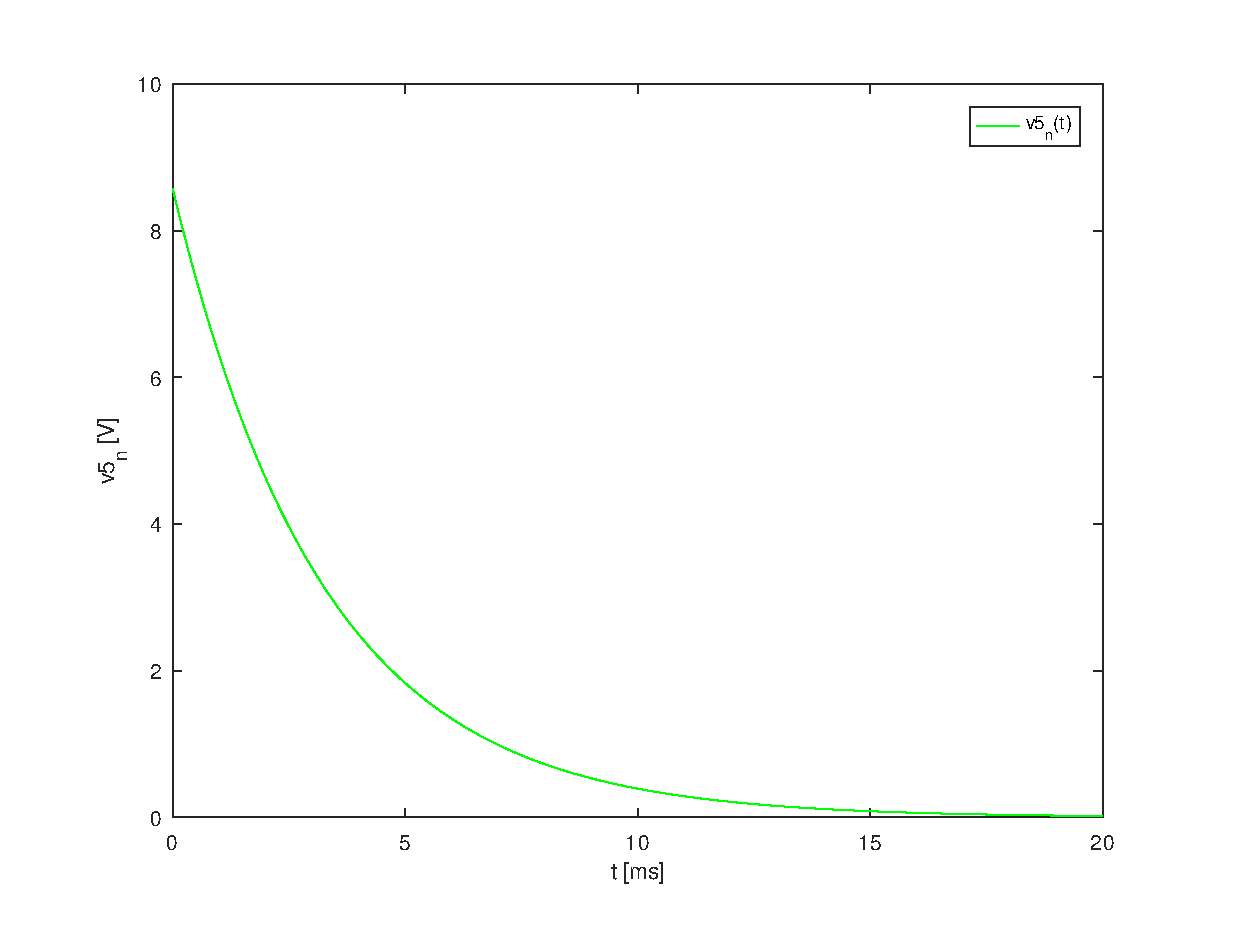
\includegraphics[scale=0.35]{v5_n.eps}
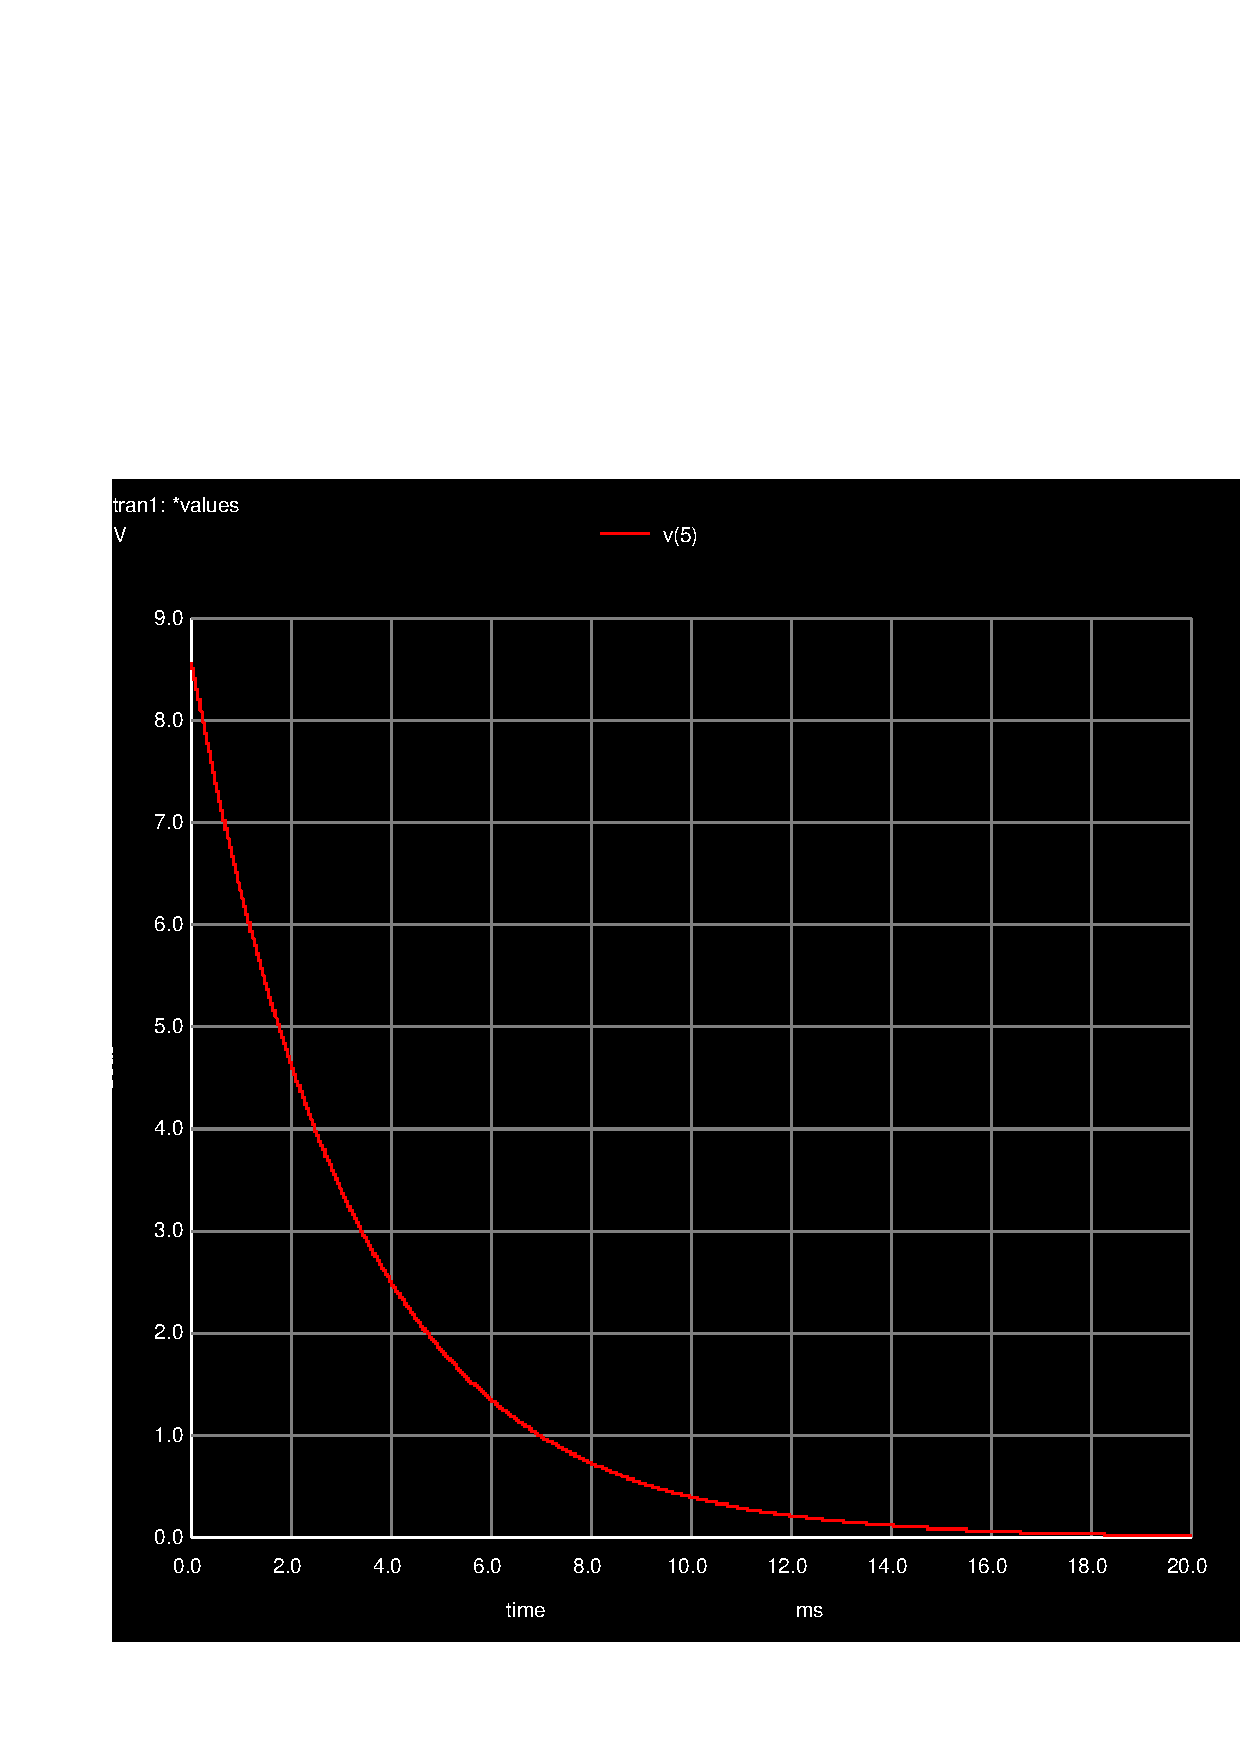
\includegraphics[scale=0.27]{transv5n.pdf}
\caption{Natural solution $v_5$}
\label{fig:comparison3}
\end{figure}
\FloatBarrier

\subsection{Final solution}
%Tudo identico aqui também, as amplitudes e fases estão de acordo entre o Octave e o NgSpice. Possivel ver que a amplitude de V5 total nunca muda, tal como se viu no ponto 2.4 apenas a parte natural interfere no decréscimo de tensao que 5 tem ao longo do tempo. E verifica-se com sucesso que o Vs tem aplitude constante e fase constante também. Tal como esperado as fases nao coincidem entre o V5 e o Vs
% isto nao sei se fica melhor aqui ou nalgum ponto mais acima.

\begin{figure}[h] \centering
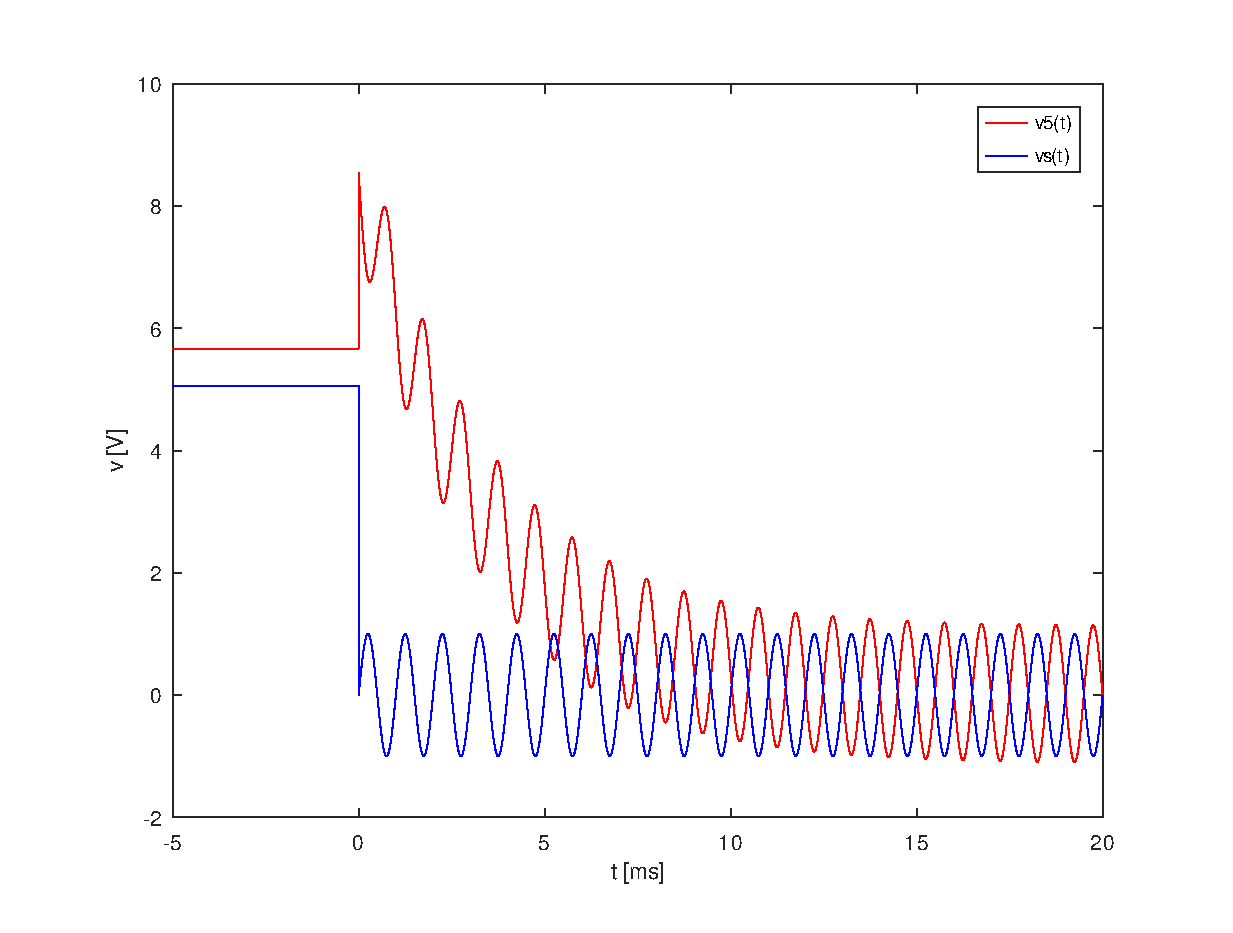
\includegraphics[scale=0.35]{v5_vs.eps}
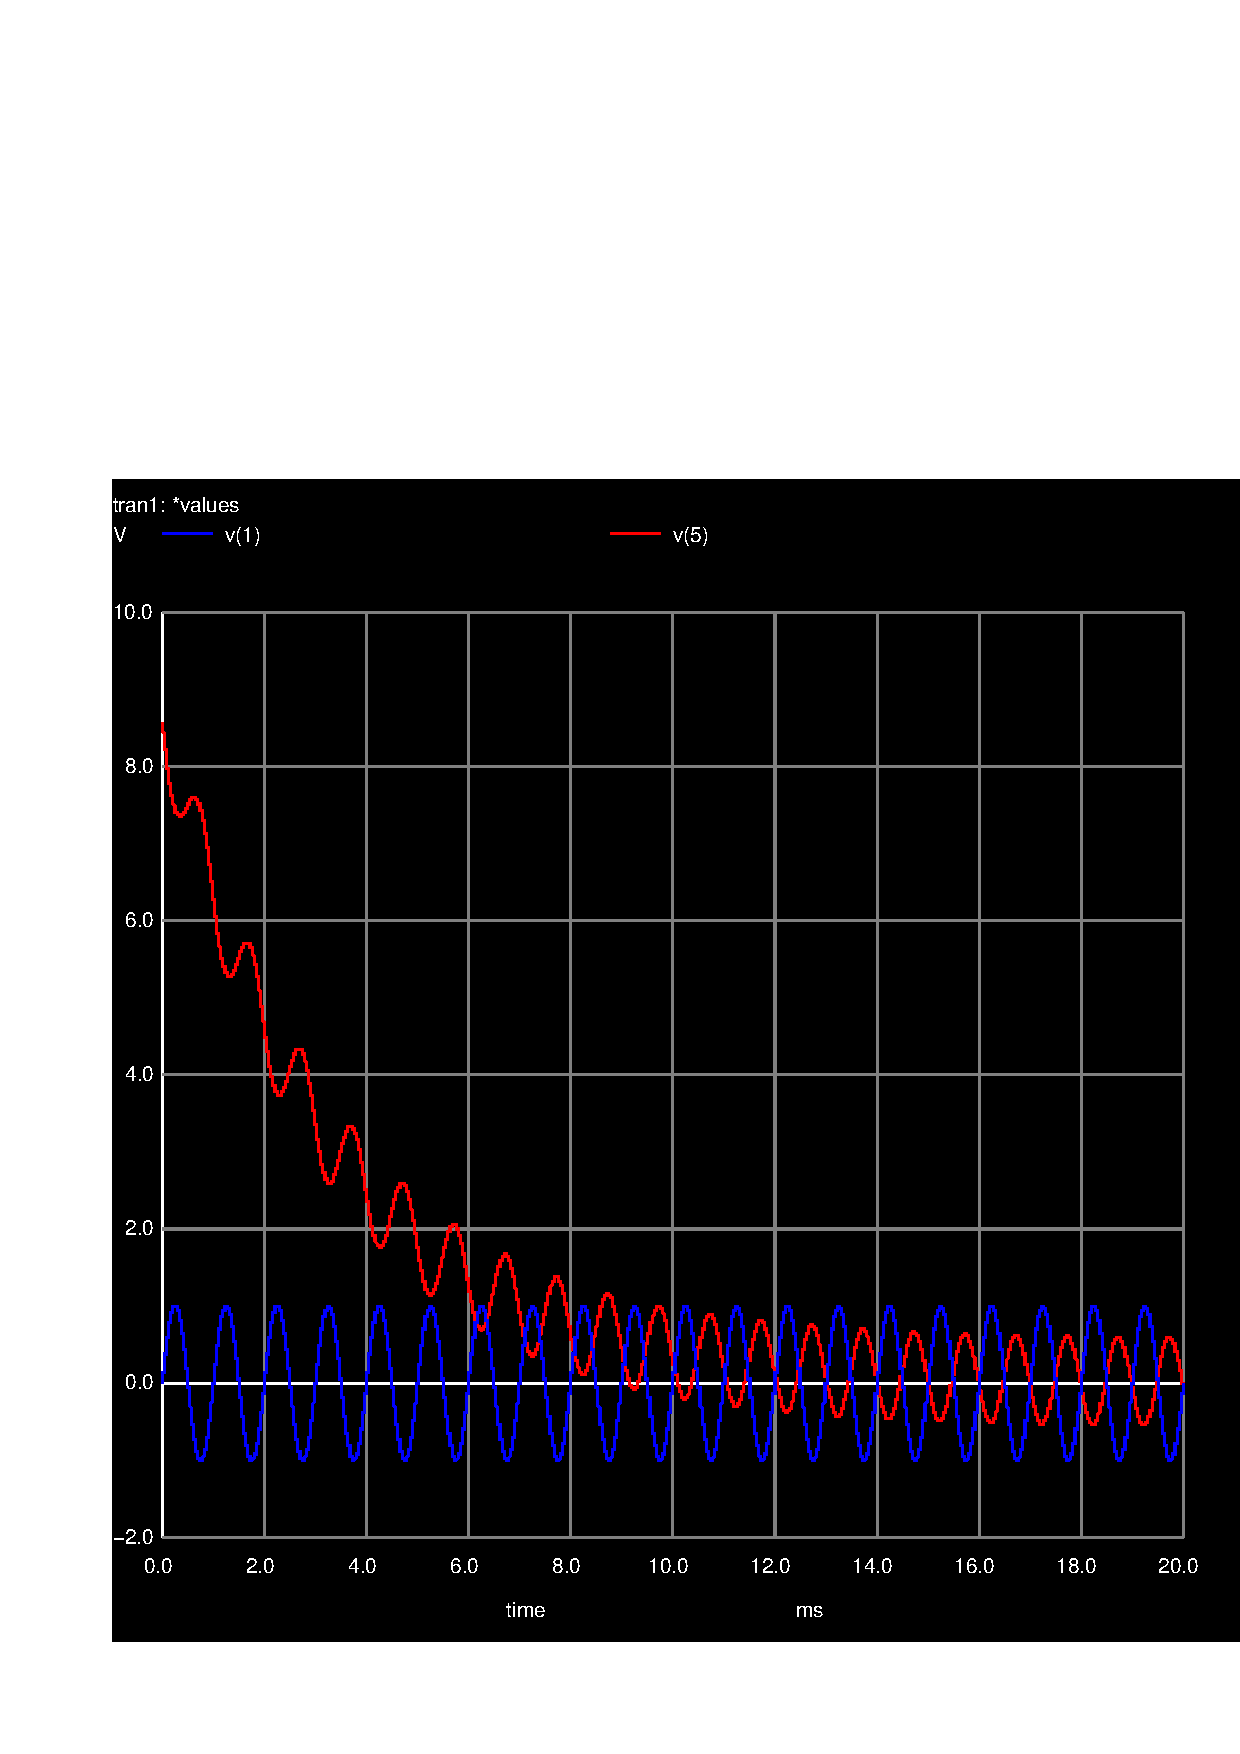
\includegraphics[scale=0.27]{transv5vs.pdf}
\caption{Final solution $v_5$ and $v_s$}
\label{fig:comparison4}
\end{figure}
\FloatBarrier

\subsection{Frequency response}
%Aqui é onde está a dúvida mas os gráficos do Octave e Ngspice são idênticos.

\begin{figure}[h] \centering
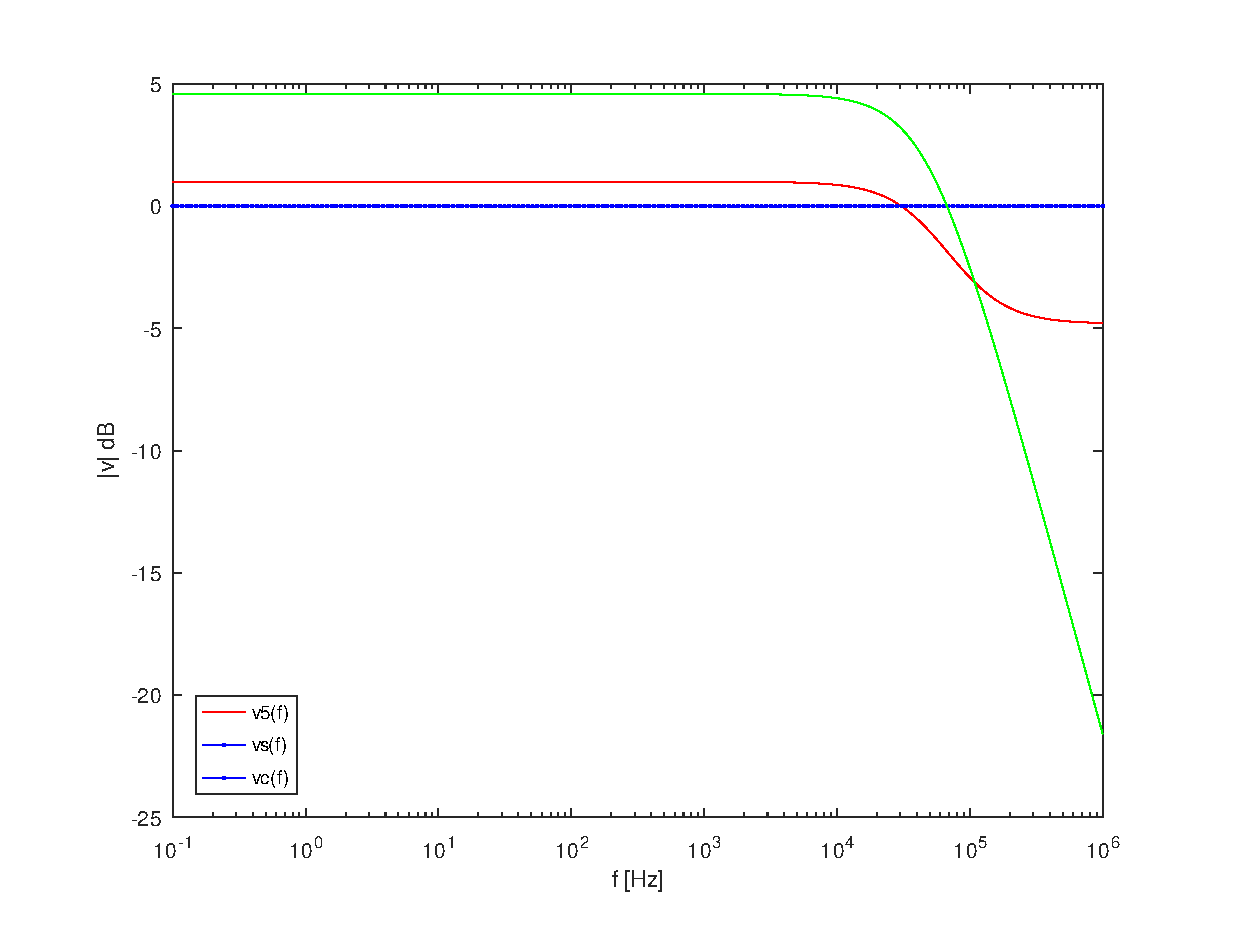
\includegraphics[scale=0.35]{freqresp.eps}
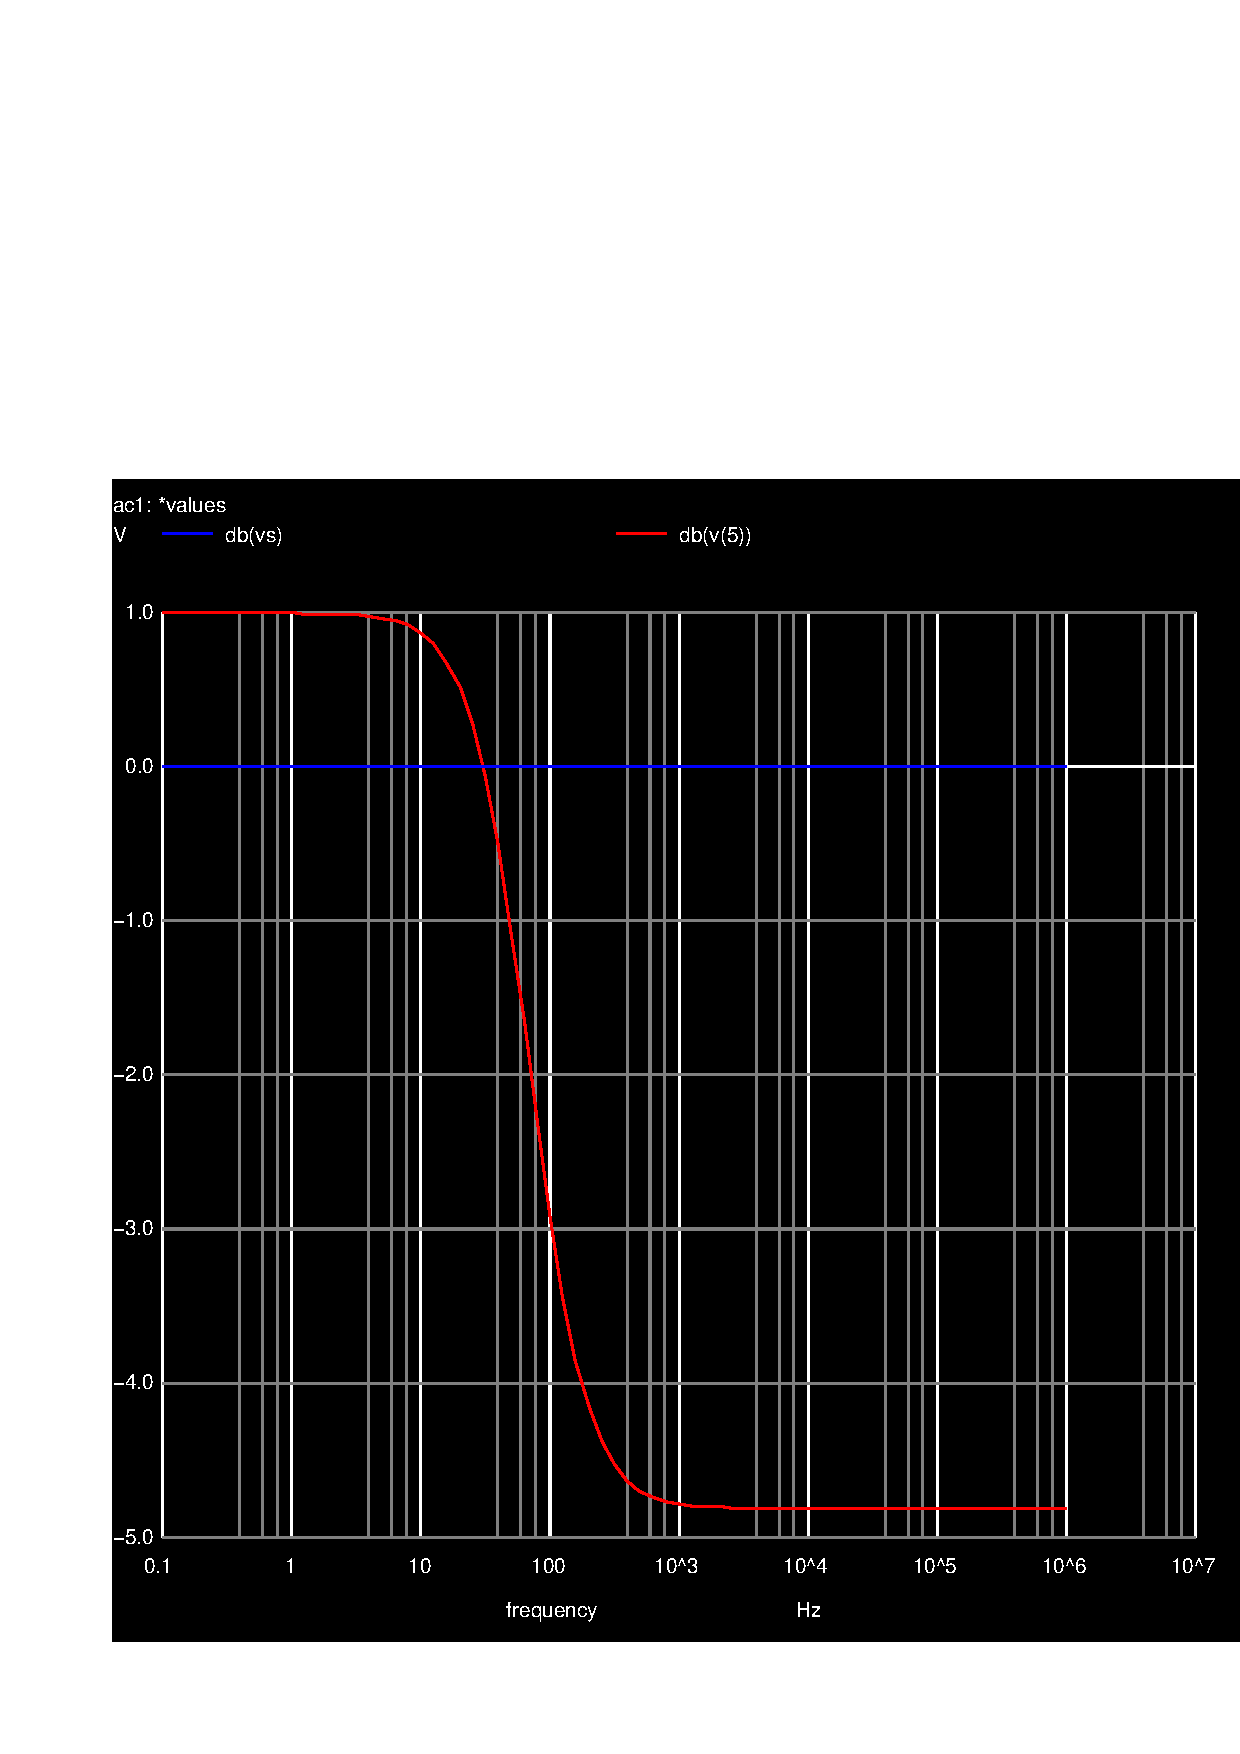
\includegraphics[scale=0.27]{db_v5_v1.pdf}
\caption{Magnitude in dB}
\label{fig:comparison5}
\end{figure}
\FloatBarrier

\begin{figure}[h] \centering
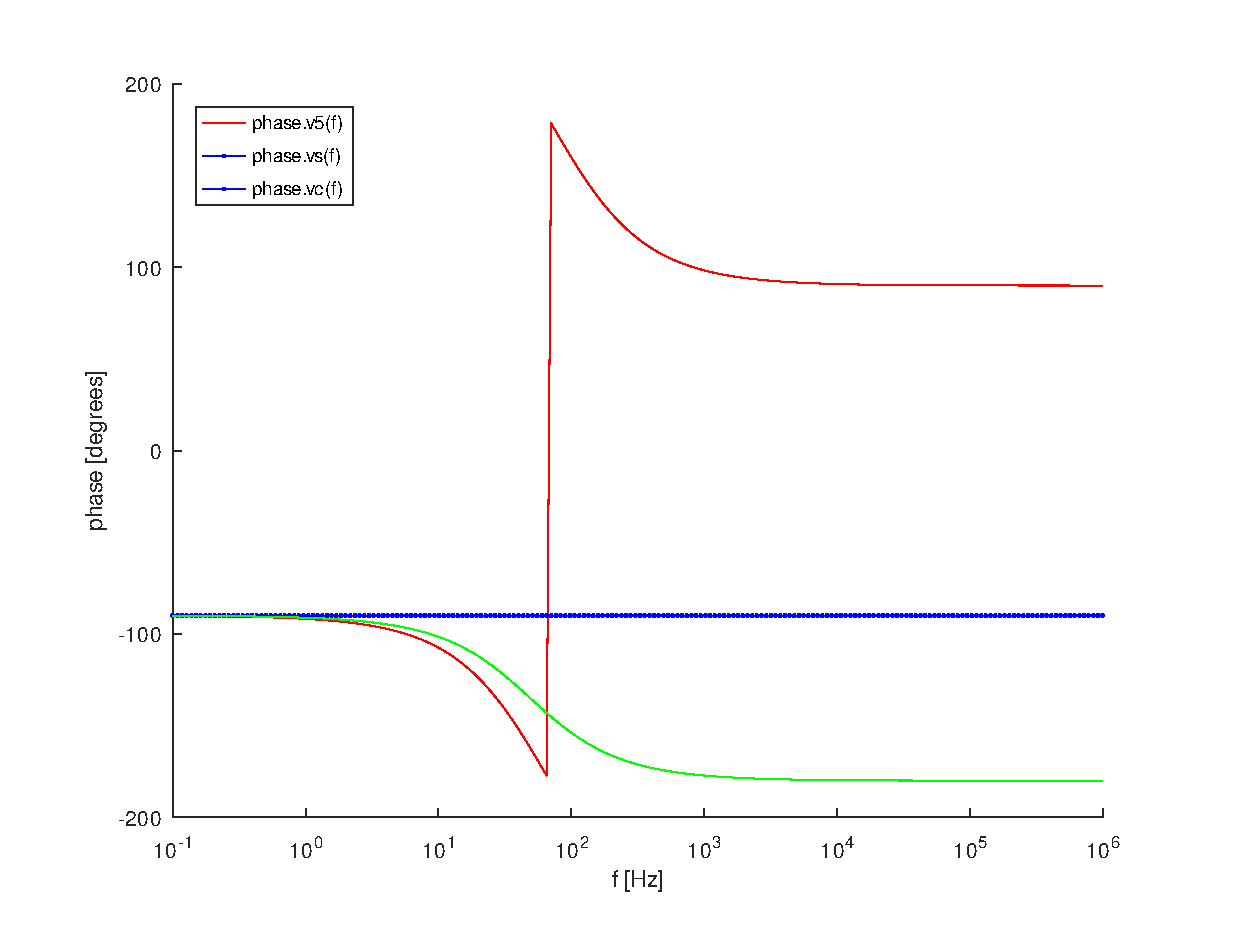
\includegraphics[scale=0.35]{phase_oct.eps}
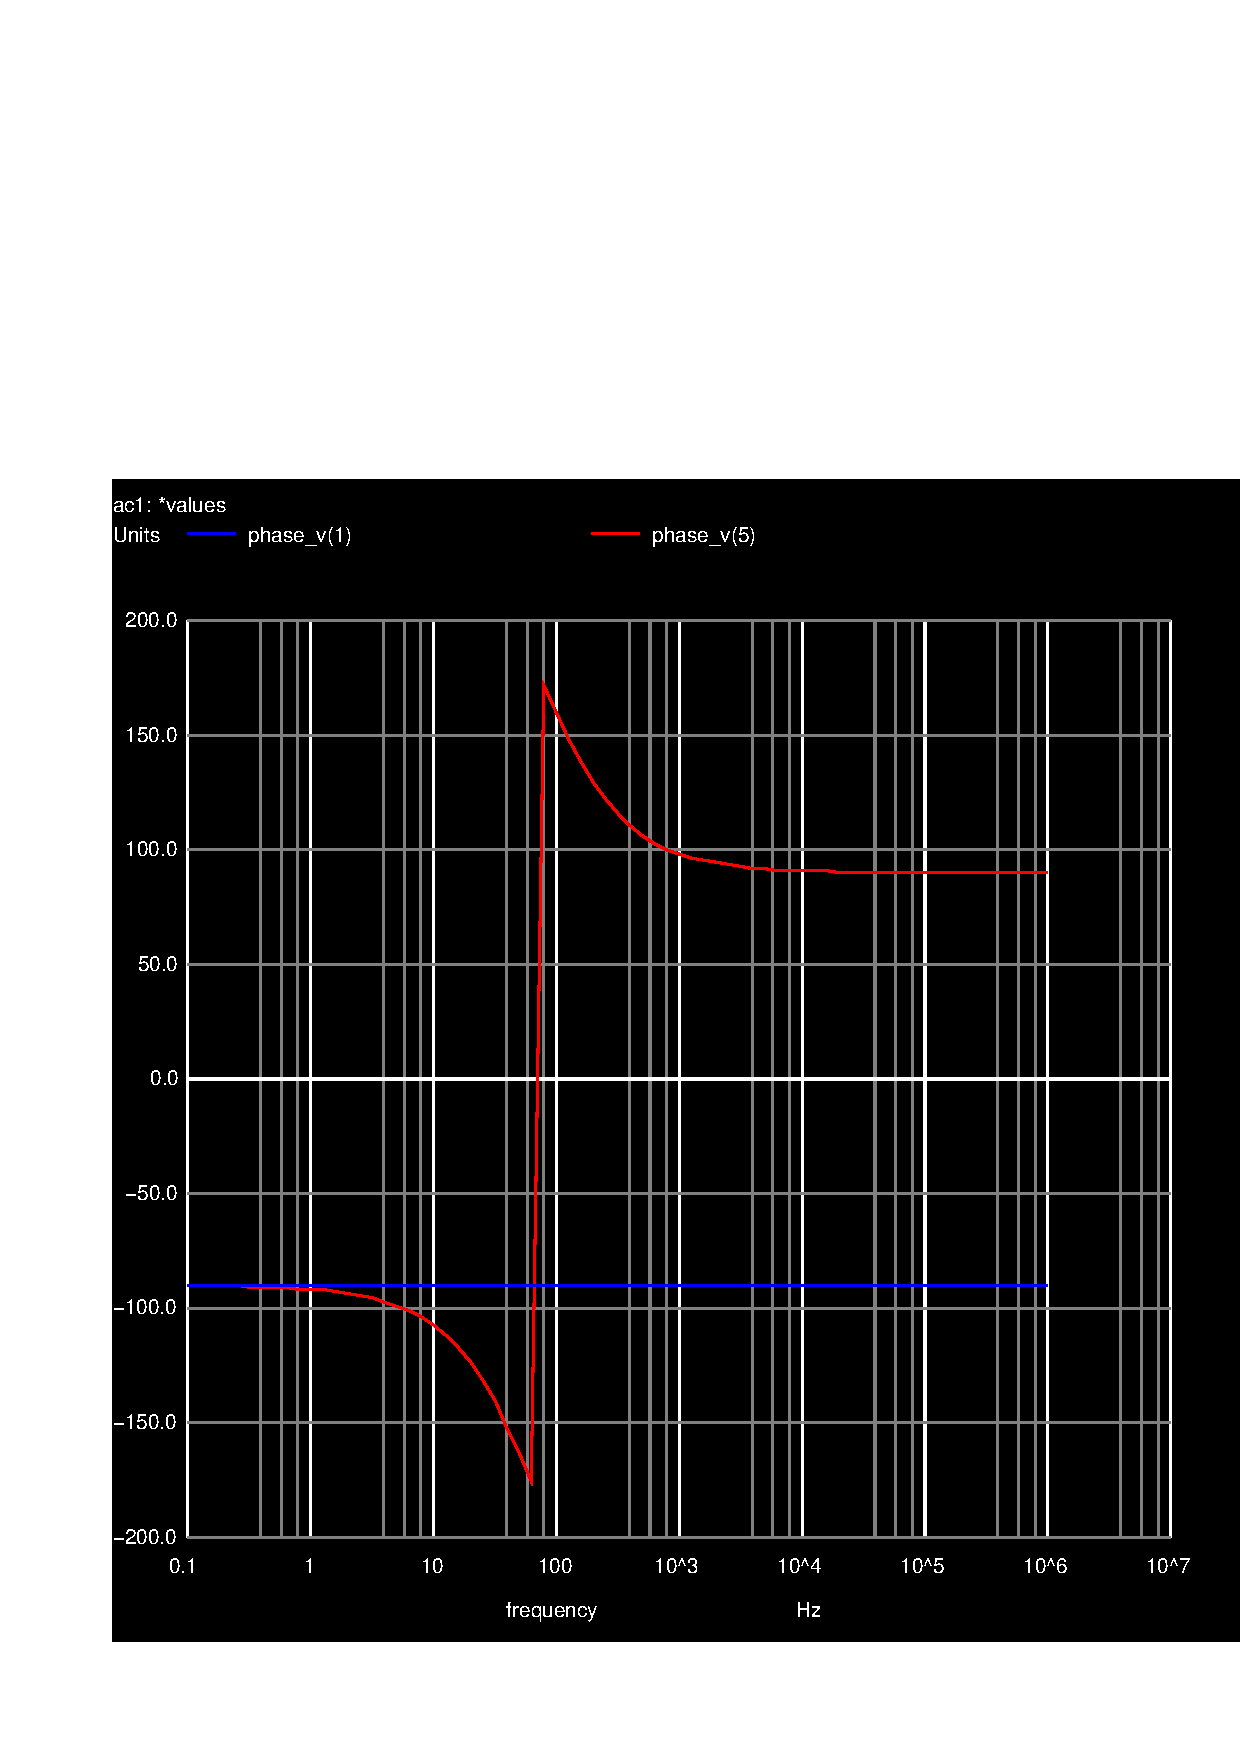
\includegraphics[scale=0.27]{phase.pdf}
\caption{Phase in degrees}
\label{fig:comparison6}
\end{figure}
\FloatBarrier


